%!TEX root = ../template.tex
%%%%%%%%%%%%%%%%%%%%%%%%%%%%%%%%%%%%%%%%%%%%%%%%%%%%%%%%%%%%%%%%%%%%
%% chapter4.tex
%% NOVA thesis document file
%%
%% Chapter with lots of dummy text
%%%%%%%%%%%%%%%%%%%%%%%%%%%%%%%%%%%%%%%%%%%%%%%%%%%%%%%%%%%%%%%%%%%%
\chapter{Implementation of the \textit{iCBD-Replication and Cache Server}}
\label{cha:impl_replication_caching}

This chapter addresses the implementation of the central topics of this thesis, divided into two major fields.
We first start with a section talking about the creation of a middleware system that provides replication features in an integrated way to the iCBD platform. While providing a detailed description of the concept and architectural model, as well as the implementation decisions, made along the accomplishment of this contribution.
Next, we show the work done on improving the performance of the platform clients. Displaying how setting up a client-side caching system that stores images adjacent to the consumers obtain that sought enhancements. Concluding in exploring the challenges of recreating the complete platform in a new environment and implementing a real-world scenario at Nova University Computer Science department laboratories.

%will at last state the problem and motivation for introduction replication techniques in the storage components of the platform. Moreover, the section prefaces the importance of the implementation of cache servers that hold part of the distribution burden and crucial for the support of an increased number of clients.

This chapter is partitioned as follows :

\begin{description}
    %
    \item [Section~\ref{sec:impl_icbdrep}] overviews the implementation of the middleware dubbed iCBD-Replication. Beginning the journey through the initial architectural process and then showing the implemented components and their interaction with the several layers of the platform.
    %
    \item [Section~\ref{sec:impl_cache_server}] shows how the complete iCBD platform was installed in the NOVA University cluster. Then, a description of the work performed to include a client-side caching server directly connected to the final clients.
    %
\end{description}
\newpage



%%-------------------------------------------------------------------
%%	4 - Implementation of a Replication Module
%%-------------------------------------------------------------------
\section{Implementation of a Replication Module}
\label{sec:impl_icbdrep}

One of the central objectives of iCBD is to provide a platform that can be both cloud-centric, with the administration and a portion of the storage burden gathered in a public cloud, or fully hosted on client premises. Either way, it becomes evident that data locality is an important subject, which means that there is the necessity to study how this data will flow between the multiple components of the iCBD platform.
As can be imagined, this is a data-intensive platform, boasting multiple storage devices in many networks and an array of consumers demanding that data at any given time.

All these factors allied to the platform architecture result in the need to create a new component, whose chief mission is to ensure that the data is correctly replicated in the appropriate places, maintaining the consistency of the various versions of the iCBD Machine Images stored.



%%-------------------------------------------------------------------
%%	4. - Requirements of the Module
%%-------------------------------------------------------------------
\subsection{Requirements of the Module}
\label{sub:impl_requirements_icbdrep}

Since the beginning of this work, the file system selected for use in the storage layer was selected, this is due to the fact that, there was already a functioning prototype of the core iCBD platform making use of BTRFS for all data storage matters. The most critical feature for the operation of the platform is that the file system supports snapshots. BTRFS is a modern file system based on the copy-on-write (COW) principle capable of creating lightweight copies of a file. We detailed the importance of this trait in Section~\ref{sub:icbd_storage_layer}.
% TODO Cap4 Requirements Citation needed on COW
 
The condition described above applies only in the choice of the File System, in theory, any File System that supports snapshots can be employed in the platform. That is, in fact, the case with the work developed in a dissertation carried out in parallel to this one, where the focus is the use of an object-oriented file system, in particular, the CEPH File System.
Due to this imposition, it is key that this work makes the best use of the BTRFS features, exploring the incremental backup capabilities. More, the replication process should fully integrate with the core platform that already distributes iMIs to clients. Preservation of consistency of the iMIs is also a concern, assuring the distribution of new versions when they are created.

Moreover, it should be taken in account the locality of the data, since the communications could originate and end in the same data centre and the same local network, or happening between different locations that can be in opposite sides of the world. Such aspects as the bandwidth used and the encryption of the data becomes essential to address, requiring the examination of several compression algorithms that can be accommodated to the way the data is processed and also ways of keeping this data secure by encrypting the communications.
\newpage

%Requirements
%The file system is set BTRFS will be used.
%Many reasons for that:
%The most important is the support for snapshots
%Compression


%\subsubsection{Preliminary tests on the BTRFS Incremental Backup features}
\paragraph{BTRFS Incremental Backup feature}
\label{par:impl_incremental_btrfs}

A first step is trying to understand the most efficient way to transfer this unique kind of data (i.e. an iMI). Given the fact that we are working with a file system with snapshots capabilities, we want to take advantage of this functionality and minimise the amount of data roaming the network.

The BTRFS developers provide a userspace set of utilities that can manage BTRFS filesystems, called \texttt{btrfs-progs}. Within that set of tools, there is a pair of commands, \texttt{btrfs send}~\cite{btrfs_send}, and \texttt{btrfs receive}~\cite{btrfs_receive}, that provides the capability to transport data via a stream and employ those differences in a remote filesystem. 

The send command facilitates the process of generating a stream of instructions that describe changes between two subvolume snapshots. Also available in the command is the ability to use an incremental mode, where given a parent snapshot that is available in both send and receive sides, only the small delta between snapshots (e.x. \textit{V2} and \textit{V2-1} in fig~\ref{fig:imi_snap}) is going to integrate the stream. This feature is outstanding since considerably reduces the amount of information that needs to be transferred to reconstruct the snapshot in the receiving end. The send side operations occur in-kernel, beginning by determining differences within subvolumes and based on those differences the kernel generates a set of instructions in a custom formulated stream.

\begin{figure}[htbp]
    \centering
    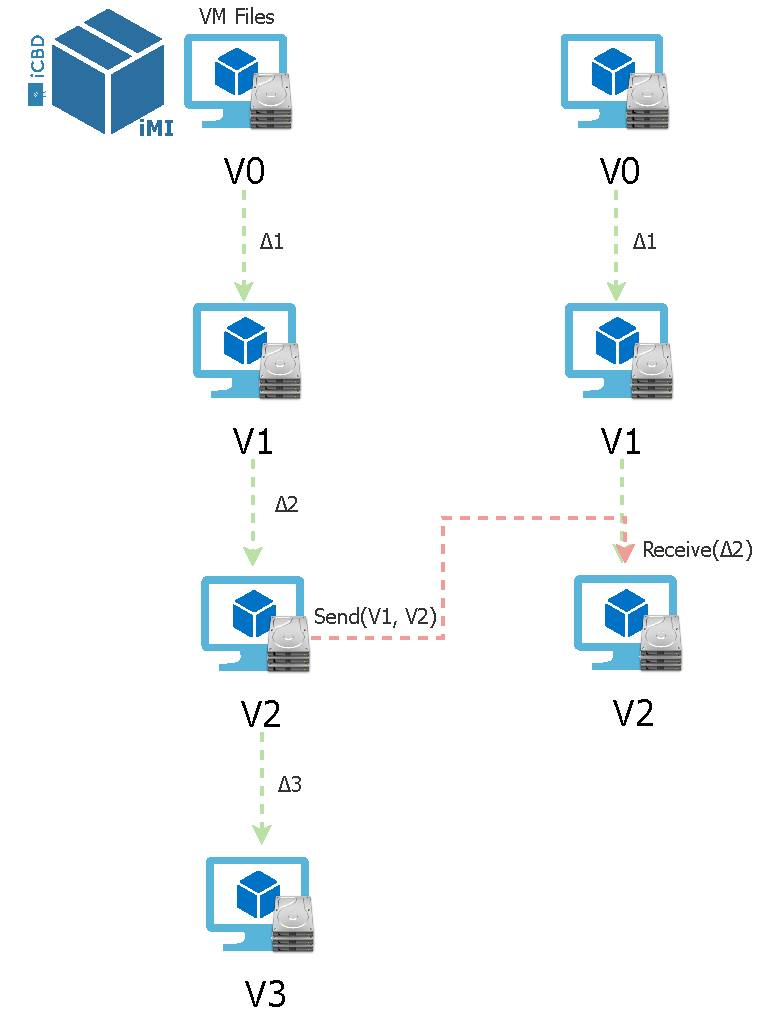
\includegraphics[height=4in]{cap4_iMI_deltas}
    \caption{iCBD iMI Snapshots Structure}
    \label{fig:imi_snap}
\end{figure}
\newpage

On the remote end, the received command accepts the stream generated by the send command and uses that data to recreate one or more snapshots. Contrary to the send command, receive executes in user space, replaying the instructions that come in the stream one by one, these instructions include the most relevant calls found in a Virtual File System, with Unix system calls like \texttt{create()}, \texttt{mkdir()}, \texttt{link()}, \texttt{symlink()}, \texttt{rename()}, \texttt{unlink()}, \texttt{write()}, along with others.~\cite{btrfs_design}


%https://btrfs.wiki.kernel.org/index.php/Incremental_Backup
%https://www.samba.org/ftp/rsync/rsync.html

%The first step is to try to understand the most efficient way to transfer this peculiar kind of data. Given the fact that we are working with a file system with snapshots capabilities, we want to take advantage of this functionality and minimise the amount of data roaming the network. In this sense, we next present some preliminary tests in multiple ways of transferring snapshots between BTRFS file systems both in the same machine and in different ones.
%The results obtained here conjugated with the defined requirements are essential for defining the architecture of the replication module steering the implementation at its best path.

%Before the start of any implementation, there was the need to validate the capabilities of the BTRFS file system regarding sending snapshots across different systems.
%As one of the requirements was the efficiency of the transference of data. So a small comparison was in order. 



%%-------------------------------------------------------------------
%%	4. - System Overview
%%-------------------------------------------------------------------
\subsection{System Overview}
\label{sub:impl_system_overview}


\begin{figure}[htbp]
	\centering
%	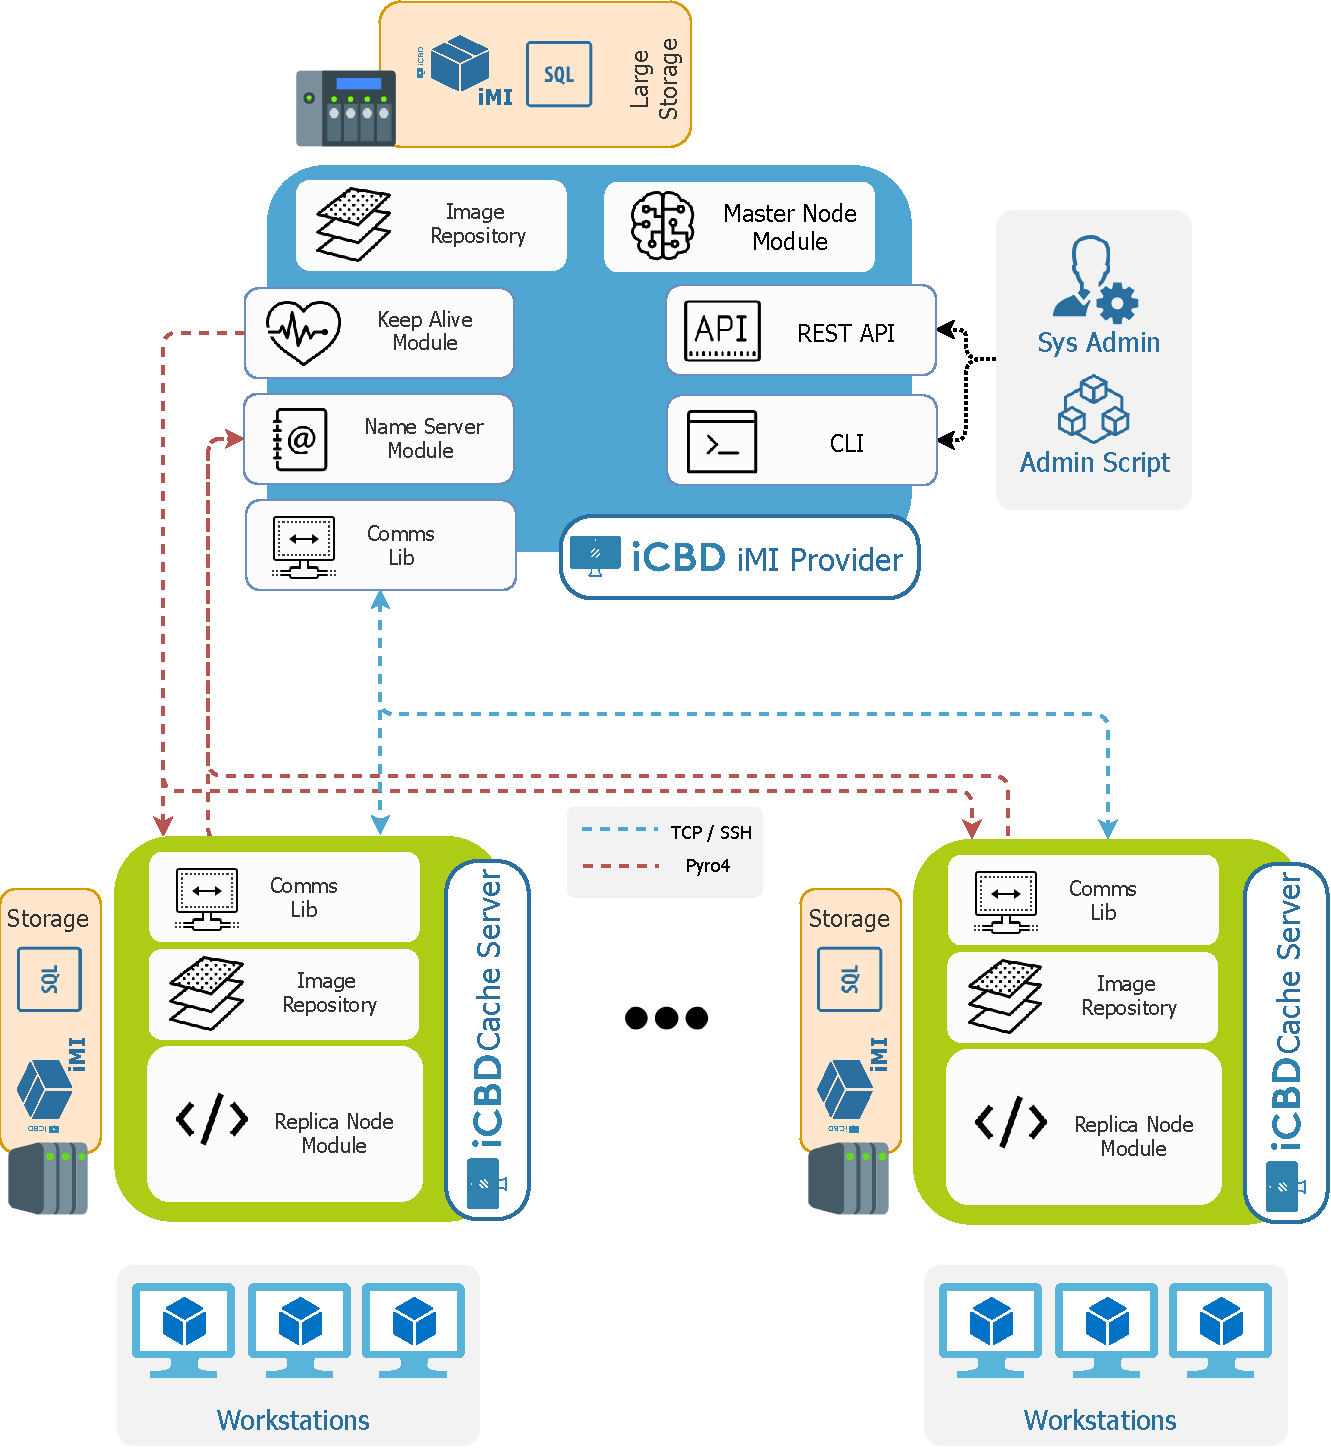
\includegraphics[height=4in, width=\textwidth]{cap4_icbd_arquit}
	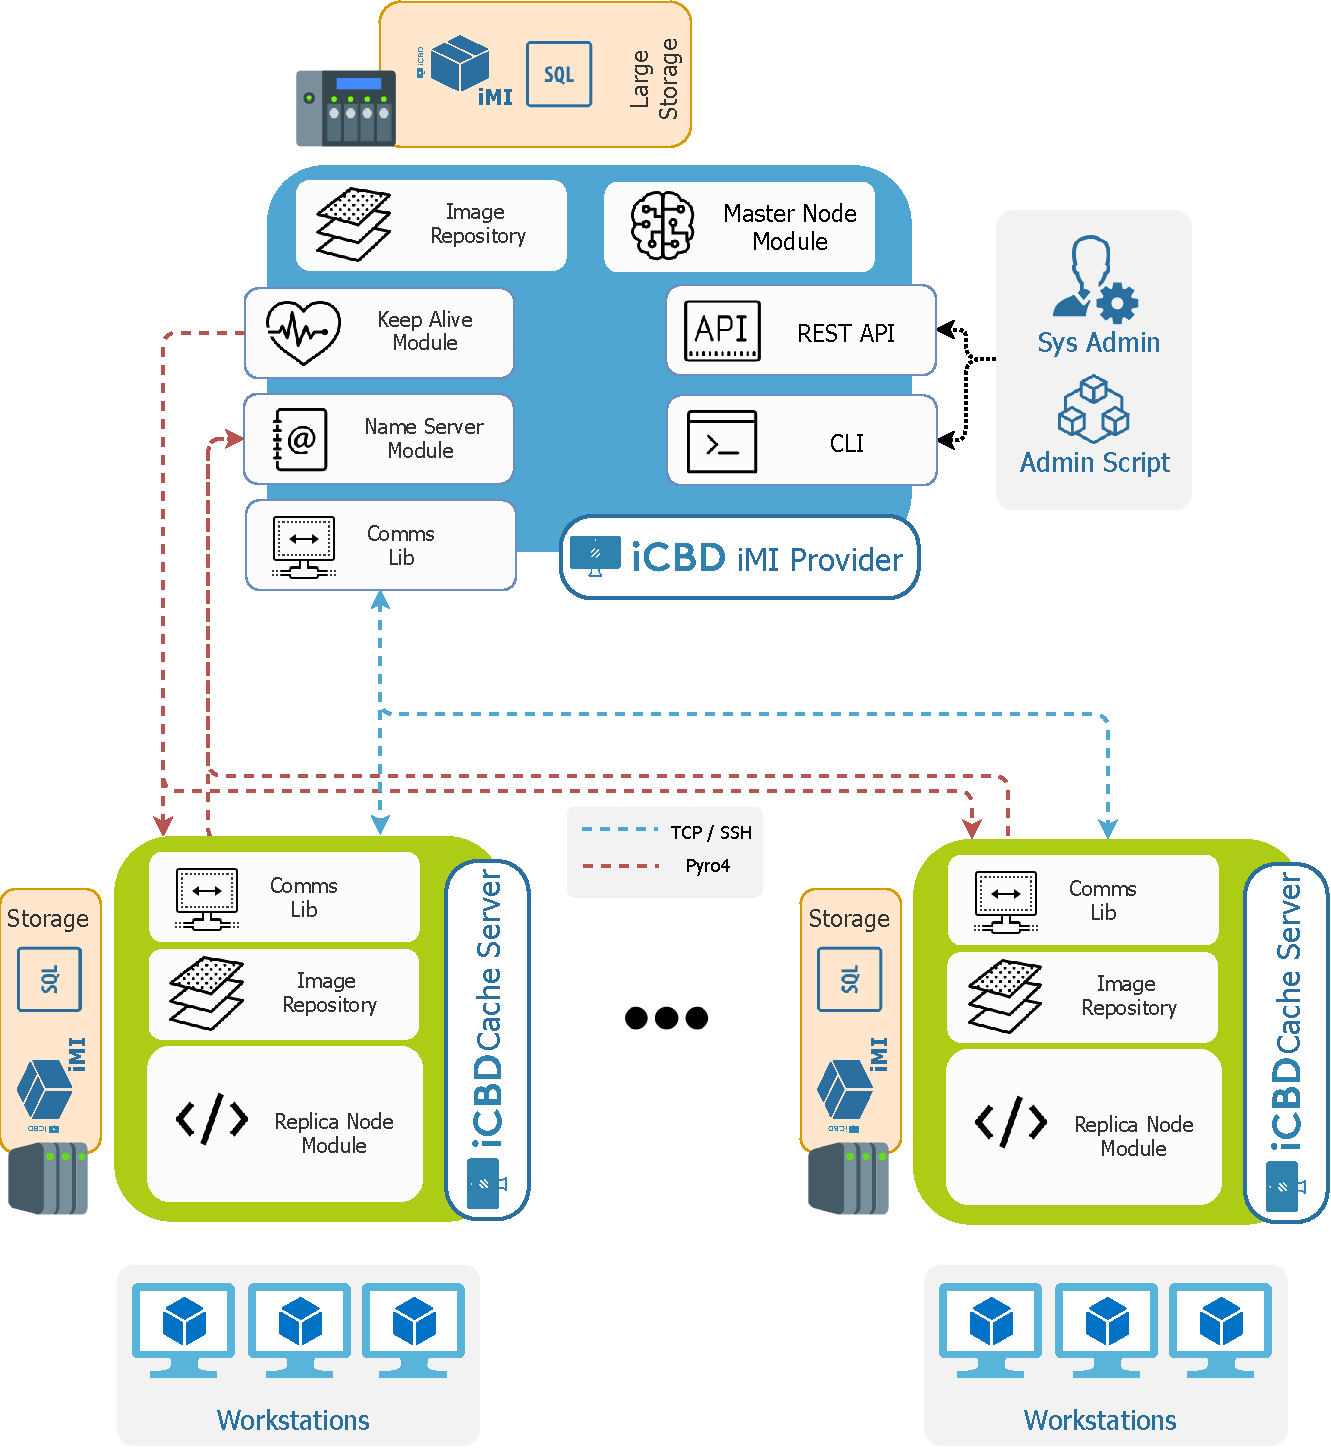
\includegraphics[width=\textwidth]{cap4_icbd_arquit}
	\caption{iCBD Replication Architecture}
	\label{fig:icbd_rep_architecture}
\end{figure}

% TODO - Cap4 System Overview - Falta referir que foi efectuada uma primeira implementação em bash script 
Since the replication module needs to interact with several bash scripts, with the core iCBD platform, including command line tools and some operating systems low-level features, we betted that the most suitable approach was creating a python distributed middleware using a master-replica paradigm.

Python as a programming language enjoys some valid idiosyncrasies, functioning as an object-oriented language, possessing an extensive standard library and enjoys a big community delivering packages with a wide range of functionality, all facts that contribute to make it the best programming language to bundle everything together.

The several modules of the middleware comprise the main functionalities allowing a node to behave as a Master or Replica node, where each one maintains its individual Image Repository. Then there are also a number of libraries that were developed to interface with some tools, as the BTRFS tool talked about above~\ref{par:incremental_btrfs}, to interface with an SSH connection, build wrappers for compression algorithms and even provide a REST API.

An overview with a small description of the functionality of each component of the system follows:

\begin{description}
	\item [Master Node] This node acts both as a controller to the replication system and an interface to interact with a client whether through a CLI or REST API. Is required that this node reside on an iCBD Administration machine since this is the node that will send changes made to an iMI to all replicas. It is also responsible for providing a communication interface with the Name Server, in this sense when an administrator wants information about which nodes are present on the platform, or what is their status; these requests obtain a route through the master node.
	%
	\item [Replica Node] The main task of this node is to maintain the subscribed list of iMIs updated, receiving the last version of those machine images and store them in the file system as soon as the Master Node makes the available. At request, the Replica Node can deliver the list of iMIs that is storing (including and very important the version numbers of the iMIs present in the node). As well as at any time subscribe to a new iMI which from that point forward will include the roster.
	%
	\item [Name Server] The name server service will run parallel to the Master Node, holding a phone book style record listing all the nodes in the replication system. Nodes register themselves in the name server during the startup process, and at any moment can query the location of another node. All this information is deposited in a simple database.
	%
	\item [Keep Alive] The keep-alive module consists of a thread, launched by the master node, tasked with periodically check if the replica nodes are still working correctly. When its identified that a replica node stopped responding, this service immediately sends a request to the Name Server for the removal of the dead node from the directory.
	%
	\item [Image Repository] This module is a custom-made data structure to hold a large set of iCBD Snapshot objects in a \texttt{key:value} store. In addition to storing these objects, provides an interface to quickly know which iMIs are store within the node that accommodates the repository. Every node in the platform (i.e. Master or Replica) must necessarily launch one repository.
\end{description}


So that all the components presented above can function adequately, they require help from several libraries. A description of those implemented libraries ensue:

\begin{description}
	\item [BTRFS Lib] The BTRFS library holds two classes. The first, called \texttt{BTRFS Tool} that is a python wrapper for the \texttt{btrfs-progs} tool, described in section~\ref{par:impl_incremental_btrfs}. The second, designated \texttt{BtrfsFsCheck} implements functions to validate if a given path is part of a BTRFS filesystem, case its true is also possible to verify if that path comprises a subvolume. Additionally, this tool is provided with a method to discover all snapshots in a directory.
	%
	\item [Compression Lib] Since multiple compression algorithms are used, makes all the sense to create a library that encapsulates multiple wrappers, one for each algorithm. These wrappers in reality only need to provide compression and decompression methods for a stream of data, with the remaining operations not present.
	%
	\item [Serialiser Lib] Some of the communications between nodes require the transmission of objects, to that effect a library containing serialisation and deserialisation methods for those objects is a requirement.
	%
	\item [SSH Lib] This library implements a wrapper for the SSH command, allowing the creation of a tunnel so that data can be funnelled through a secured connection between nodes in different networks.
	%
	\item [REST API Lib] To comply with one of the objectives of the replication module, a REST API should be provided. That is precisely what this library does, providing the endpoints to interact with the system. Also enabling an easy way to expand that interaction to other modules of the platform.

\end{description}

Even though the libraries presented above are not enough for the correct implementation of the all functionalities of the replication module, more libraries implemented by the community were necessary to handle aspects like communication between nodes, algorithms for data compression and to secure the data transmission between networks. Some of which we describe below and through the remaining text detailing each module.


%%-------------------------------------------------------------------
%%	4. - Communications between nodes
%%-------------------------------------------------------------------
\subsection{Communications between nodes}
\label{sub:impl_rep_comms}

Coordinate the multiple modules and its activities, demands from the middleware a need to share a communication channel connected through a network. 
The remote procedure call (RPC) brings support for inter-process communication allowing a procedure on a system to invoke an operation running in a process in a different location, most likely on a remote system.

As seen in figure~\ref{fig:icbd_rep_architecture}, multiple processes are running in different machines any given time, and those processes need to continually send and receive information: perhaps operations to execute, metadata updates, or just monitoring if a process is running according to the desired plan or is in a faulty state.
Managing the nodes is a perfect case for the use of the Pyro 4 library, that gives a holistic view of the system and allows triggering a multitude of operations in each node.


%\subsubsection{Pyro4 Library}
\paragraph{Pyro4 Library}
\label{par:impl_pyro4_lib}
%https://pythonhosted.org/Pyro4/
Pyro 4~\cite{pyro4} is a library that enables the development of python applications in which objects can talk to each other over the network through the use of RPCs. Its designed to be very easy to use and integrate into a project and at the same time provide considerable flexibility. This library can be imagined as an adhesive to integrate various components of a heterogeneous system easily.

There are some core features employed in the iCBD replication module, but not limited to:


\begin{description}
	\item [Proxy] This object acts as a substitute for the real one, intercepting the calls to a given method of that object. Then through the Pyro library, the call is sent to the actual object that probably resides in a remote machine, also returning the resulting data of the call. Which is very useful considering that the function that performs a call to the object does not need to know if it is dealing with a normal or a remote object.
	%
	\item [Pyro object] A Pyro object is a regular python object that goes through a registration process with Pyro in order to facilitate remote access to it. Objects are written just as any other piece of code, but the fact that Pyro knows its existence allows calls to that object that may originate in other programs.
	%
	\item [Pyro daemon] This component is the one that listens for remote method calls done to a proxy, dispatches them to the real object and collects the result of the call returning it to the caller.
	%
	\item [Name Server] Is this tool that keeps track of the objects actual locations in the network so they can move around freely and transparently. Works similarly to a yellow-pages book, providing lookups based on metadata tags.
	%
	\item [Automatic reconnecting] If a client (in our case a Replica Node) becomes disconnected to the server (Master Node), because of a server crash or a communications error, there is an automatic retry mechanism to handle this fault.
	%
	\item [Secure communication] Pyro itself does not encrypt by default the data it sends over the network. Still, Pyro RPCs communications can travel over a secure network (VPN, SSL/SSH tunnel) where the encryption is taken care of externally to the library. Alternatively, it is also possible to enable SSL/TLS in the Pyro library itself, securing all communications with custom cert files, private keys, and passwords.
	%
	\item [Serialisation] Pyro supports the transformation of objects into streams of bytes that flow over the network to a receiver that deserialises them back into the original format. This process is essential to ensure the delivery of all data that remote method calls receive as arguments, as well as the corresponding responses.
\end{description}


\paragraph{TCP Sockets and Secure Shell Protocol (SSH)}
\label{par:impl_tcp_sockets_ssh}
Despite the facts presented above, system coordination is not all the burden laid on the network, the main task of this system is to replicate virtual machine images among the several nodes, so the network also has responsibility on carrying large volumes of data (result of transferring iMIs). The Pyro4 library gives the possibility to secure its communications, but that only covers method calls within replication nodes. 

The delivery process of iMIs throughout nodes follow one of two principles: in the first scenario, we consider the case where the iMI does not leave the same trusted local network (i.e. communications within the walls of one organisation); the second implies the transport of data between third-party networks, even the internet. 

When talking about an organisational network, it's safe to assume that there are some security measures already in place (e.g. VLANs), so in this regard, we transfer the concerns about data security for that layer. That fact allows the use of a simple Stream Socket~\cite{py_socks} which provides a connection-oriented flow of data with error detection, in our case implemented on top of TCP. The application of this type of socket and the non-use of cyphers allows the best performance in the transfer of an iMI without the addition of computationally heavy tasks such as encrypting a large amount of data.

In the second case, to solve the question of the data travelling through open networks, an extension of the previous solution is presented, using the same type of socket but redirecting the flow through an SSH tunnel deployed between nodes. 

This solution in addition to solving the issue of ensuring data security in the transferal process is a modular solution that allows future changes in the way data is encrypted without needing significant modifications to the code base. Even so, we do not believe that this is a perfect security model, there is room for improvement, but, not being the focal point of this work, we still wanted to provide some security features for conducting functional tests linking geographically separated data centres.



\paragraph{Data Compression}
\label{par:impl_data_compression}

Following one of the requirements stated above, our work should aim for reducing the bandwidth consumed by the operations of the iCBD platform, and that includes the replication of iMIs. Part of this subject is already addressed in the Storage Layer since the images, by default, are transparently stored in BTRFS compressed with zlib~\cite{btrfs_compression}. However, the replication process using the BTRFS send and receive features, as explained in section~\ref{par:incremental_btrfs}, does not send the iMIs as is, send an instruction stream, and those instructions present as an excellent candidate to be compressed. 

Given the design of the send \/ receive feature, is unthinkable to hold in memory all the instructions waiting to be compressed, or store that information in a file, compress it an then send without creating a huge bottleneck and introducing a delay on the replication process. To expedite the process of transmitting the stream compressed and without postponements, only compression algorithms that provide a framing format (i.e. allowing compressing streams that can then more easily be decompressed without having
to hold the entire stream in memory) were chosen.

In this work, we included three algorithms that presented the framing format characteristic, and that demonstrated to be popular in use, but maintained a code base modular where is very easy to add a new algorithm.

\begin{description}
	\item [LZ4] is a lossless data compression algorithm centred on compression and decompression speeds, that belongs to the LZ77 family~\cite{lz77} of byte-oriented compression schemes. The reference implementation is in C and initially implemented by Yann Collet. There are also ports and bindings, from the original C implementation, in various languages like Java, C\#, Python, Go, among others. In this work, we use a multi-threadable python biding by Iotic Labs called \textit{py-lz4framed}~\cite{lz4framed}.
	%
	\item [zlib] is a widely used, kind of a \textit{de facto} standard, library of lossless data compression that uses an abstraction of the DEFLATE compression algorithm (also a variation of LZ77). The algorithm written by Jean-loup Gailly and Mark Adler provides good compression on a wide variety of data sets and environments with the minimal use of system resources.~\cite{zlib} Written in C, can be found in the most diverse platforms: used by the Linux Kernel in multiple instances, multimedia libraries, databases, version control systems, and others. In the replication module, we employ the included zlib library~\cite{py_zlib} in python which provides an interface to the zlib C library.
	%
	\item [Snappy] is a compression \/ decompression library, created by Google~\cite{snappy}, that contrary to other algorithms, strives for very high speeds at reasonable compression rates, not maximum compression. The library is written in C++ but counts with several bindings for the most popular languages. In order to interface with python, we used the python binding~\cite{py_snappy} for the snappy C++ compression library, provided by Andrés Moreira.
\end{description}

%%-------------------------------------------------------------------
%%	4. - Name Server
%%-------------------------------------------------------------------
\subsection{Name Server}
\label{sub:impl_icbdrep_name_server}

%\textbf{TOPICS :}
%\begin{itemize}
%	\item Starting Pyro4 Name Server from within iCBD-Replication code
%	\item Configurations applied (ip / port)
%	\item How the Name Server is controlled?
%\end{itemize}

In a distributed systems environment the various nodes need to know how to communicate with each other: uniquely identifying themselves and refer to there locations. The mechanism that addresses this problem is commonly referred to as Naming.~\cite{tanenbaum_2006}

The iCBD Replication module implements this feature, attributing to each node an identity tuple with three elements: \texttt{(Node Name, Node URI, Tag)} that is registered in a name server allowing for subsequent locate a node by its name, or retrieve a set of nodes that are marked by the same tag.

The name server is a module that consists of a constant running thread and a local \textit{SQLite} database. It makes use of the aforementioned Pyro4 Name Server, but instead of being launched from a console, it leverages the "launch on your code" feature provided by the library to seamlessly integrate this feature with the remaining modules and starts up together with other modules of the Master Node.

Given the scenario where a node wants to make contact to another node and does not have its location. A request with the name of the node is made to the name server expecting in return a URI to call. If the requesting node already knows the location (IP and Port) of the name server, it makes the request directly. However, in the case where it also does not know how to contact the name server, resorts to a simple UDP network broadcast to locate the name server.

\begin{listing}[ht]
\inputminted{python}{./Chapters/Code/cap4_NameServer.py}
\caption{Starting procedure of a Name Server}
\label{listing:impl_icbd_nameserver}
\end{listing}

\paragraph{Methods in the Name Server API}

The Pyro Name Server presents an extensive API, but for the purposes of our work, only the subset presented below is utilised. 

\begin{description}
	\item \texttt{locateNS()} Get a proxy for a name server somewhere in the network.
	\item \texttt{register()} Enrol an object on the name server associating the URI with a logical name.
	\item \texttt{list()} List all objects registered in the name server. The results will be filtered if a prefix is provided.
	\item \texttt{lookup()} Looks for a single name registration and returns the corresponding URI.
	\item \texttt{remove()} Removes an entry, created by registering an object, with the exact given name from the name server.
\end{description}





%%-------------------------------------------------------------------
%%	4. - Image Repository
%%-------------------------------------------------------------------
\subsection{Image Repository}
\label{sub:impl_icbdrep_image_repo}

Each Replica Node in the platform can subscribe to an independent set of iMIs that will be replicated to its local storage, with the Master Node holding the entire collection. 
To represent this relation between nodes and to facilitate the process of knowing which image is present in each node we implemented an Image Repository.

This sub-module is present in every node (Master and Replicas) and presents itself with a central role in the replication process, not only, by the fact of acting as the backbone for the subscription of images, but also by tracking all versions of iMIs present in the platform working similarly to a versioning system. As described before, the iCBD platform stores the multiple versions of one iMI as snapshots, that materialise as directories in the local filesystem. Like to what happens in the Name Server, the information stored by the Image Repository is backed in persistent storage in the form of an \textit{SQLite} database. 

The interface that the Image Repository offers is elementary, giving a hand full of mutator methods (get and set functions) to populate one main data structure. The structure used is the Python builtin Dictionary, allowing to establish an unordered set of \texttt{key:value} pairs, where the \texttt{key} is the name of the iMI and the \texttt{value} is a \texttt{List} of several \textit{icbdSnapshot} objects, one for each version.

%\subsubsection{iCBD Snapshot Object Structure (iMI)}
\paragraph{iCBD Snapshot Object Structure (iMI)}
\label{par:impl_icbdrep_snapshot}

Inside the replication module, the iMI as presented in Section~\ref{sub:icbd_imi}, is treated as a first-class citizen, being represented by the class \textit{icbdSnapshot}. This object stores the relevant metadata and properties of an iMI that are essential to distinguish the multiple images present in the system unequivocally, but do not hold actual data.

In that sense, from this lightweight object, we can obtain: the name of the iMI, its version number, the full path to the VM files in the filesystem, the location of the boot package regarding the version in question, and the configuration file for the iSCSI target. Since the data stored within this object is appended on its creation and is immutable, the object only provides \texttt{get} functions to retrieve its values.

Given that all the relevant data is stored locally in a node (i.e. the actual VM file; the boot package; the iSCSI configuration files) the \textit{icbdSnapshot} object only needs to maintain the paths to that data in relation to the local filesystem, leading to a clean and straightforward interface that can be seen in Listing~\ref{listing:impl_icbdSnapshot}.

\begin{listing}[ht]
\inputminted{python}{./Chapters/Code/cap4_icbdSnapshot.py}
\caption{Example of the information stored in the \textit{icbdSnapshot} object.}
\label{listing:impl_icbdSnapshot}
\end{listing}



%%-------------------------------------------------------------------
%%	4. - Master Node
%%-------------------------------------------------------------------
\subsection{Master Node}
\label{sub:impl_icbdrep_master_node}

%\textbf{TOPICS :}
%\begin{itemize}
%	\item Startup routine, including the launch of other services
%	\item Main controller for all nodes of iCBD-Replication
%	\item The send operation 
%\end{itemize}

Following the architecture of the replication process, one of the fundamental roles is to manage the subscription of iMIs, disseminate new versions and provide an interface to interact with it all. Given those requirements, the Master Node resides in an iCBD Administration Machine allowing to hold a particular view of all components of the system and a holistic view of the state of the platform ( i.e. identify all the nodes present in the platform, recalls all iMIs in catalogue, maintains a list with all relations between iMIs and nodes - the subscriptions). 

Moreover, adding to the above, this node also acts in a way as a gateway, delivering two methods of interfacing with the platform - a Command Line Interface (CLI) and an HTTP REST API.

More than being having a central role in managing and overseeing the several aspects of the replication platform architecture, this node holds the responsibility of sending the new versions of an iMI as they are created. This is the highlight feature that makes use of the BTRFS Incremental Backup functionality, in this case, the send operation.

\paragraph{Sending a Snapshot to a Replica Node (Cache Server)}

The general idea is: when the administration process of an iMI comes to an end, the Master Node is notified that a new version of that iMI is available. So, a new entry for that version is created and stored in the local Image Repository. Then, the main replication procedure starts. 

First, it is checked which nodes have subscribed to iMI. For those who have subscribed we need to check the latest version available in the Replica's Image Repository, this process will determine if the new version can be sent immediately, or if it is necessary to transfer some intermediate versions. 

Any of the cases, we are transmitting only the differences between versions, not the whole iMI. Assuming that only the last delta (the most recent changes) will be shipped, it is determined whether the transfer will occur using an encrypted communication channel and/or whether some compression algorithm will be applied in the data before being sent. This information is also conveyed to the receiving side so that it is ready to accept the data. 

Only after all this process begins the data transfer, being aided by the libraries mentioned above, btrfsLib; compressionLib and sshLib. The process of receiving an IMI can be found in the Section~\ref{par:impl_receive_snap}.

\paragraph{Keep Alive}
\label{par:impl_icbdrep_keep_alive}

%\textbf{TOPICS :}
%\begin{itemize}
%	\item Launched by the master node
%	\item Periodically check if the replica nodes are still working
%	\item Case any change talks to the Name Server to change things according
%\end{itemize}

There is a point mentioned when presenting the Pyro4 platform mentioned that this library allows the automatic reconnection of clients to the Master Node, however, the opposite is not provided. In case of failure of a Replica Node, the Name Server is not automatically informed of this failure, in fact, this event would only be noticed when a connection with that node failed.

Since we want the Master Node view always to be consistent with the status of the platform, it is essential that the Name Server always hold its information up-to-date. It is to satisfy this accountability that this submodule enters in the picture. Similarly to the Name Server, the Keep Alive feature is also launched in conjunction with the Master Node and also runs on its own thread, making the execution flow independent of any other sub-module.

The principal task implies verifying the activity status of all Replica Nodes, indexed by the Name Server, in a quite simple manner. Taking the list of all Replica Nodes and with a periodicity of about ten seconds, each node is reached with a style of a ping expecting a response to the challenge. If there is no acknowledgement, two further contact attempts are performed, if those too fail, it is assumed that something wrong happened to that node and is therefore declared inactive. At this point, the Name Server is reached notifying that a node entered a failed state and should be excluded from the record. 

\subsubsection{CLI Interface}
\label{subsub:impl_icbdrep_cli_interface}

One of the methods to interact with the iCBD replication platform is through a Command-line interface provided by the Master Node, which is nothing more than a program that launched from a terminal textually recognises a series of commands and returns its result.

\begin{description}
	\item \texttt{List Replicas}
	\item \texttt{Update Name Server}
	\item \texttt{List Subscribed iMIs}
	\item \texttt{Subscribe iMI}
	\item \texttt{Unsubscribe iMI}
	\item \texttt{List iMI available versions}
	\item \texttt{Send iMI Snapshot}
	\item \texttt{Send iMI Snapshot Secure Connection (SSH)}
	\item \texttt{Delete iMI version}
\end{description}


\subsubsection{REST API}
\label{subsub:impl_icbdrep_restapi}
\textbf{TOPICS :}
\begin{itemize}
	\item Flask lib
	\item Endpoints
\end{itemize}


%%-------------------------------------------------------------------
%%	4. - Replica Node
%%-------------------------------------------------------------------
\subsection{Replica Node}
\label{sub:impl_icbdrep_replica_node}

\paragraph{Receiving a Snapshot}
\label{par:impl_receive_snap}

\textbf{TOPICS :}
\begin{itemize}
	\item Operations on the local repository
	\item The receive operation
\end{itemize}




%%-------------------------------------------------------------------
%%	4. - Building a iCBD Cache Server
%%-------------------------------------------------------------------
\section{Building a iCBD Cache Server}
\label{sec:impl_cache_server}

%To solve some of the enunciated problems with a DaaS solution that derive from limited bandwidth, latency and jitter from the limitation of accessing the image repositories from an internet connection and provide some scalability feature with the implementation of proximity cache servers are key. These cache servers can store replicas of the iMIs created and maintained in an administration server. Moreover, since they are located in the same LAN segment as the clients is from here that they will boot.
%For accomplishing this work, the cache servers need to have hard drives. (Although it would be possible to have diskless cache servers, they would be blocked if there was an interruption in the internet access, and it is to avoid that the local drives are necessary. )

%A instalação, configuração e administração dos cache-servers far-se-á também pela instanciação a partir da imagem de uma VM especialmente preparada para o efeito e residente na cloud, no sistema de administração. Os cache-servers arrancam inicialmente pela rede a partir do servidor na cloud e carregam um Linux que vai formatar os discos, neles instalando o conteúdo da própria imagem de VM, terminando com a instalação de um boot loader que irá arrancar o sistema do cache-server após a máquina fazer reboot. Daí em diante o sistema de administração na cloud irá disponibilizar as actualizações que forem necessárias, podendo mesmo forçar a re-instalação total dos cache-servers.

%Note-se que uma vez instalado um cache-server numa LAN, dada a grande fiabilidade que pode ser ainda reforçada através das técnicas habituais em sistemas tolerantes a faltas e de elevada disponibilidade (referir a sugerida pelo Paulo), torna-se viável a utilização de servidores diskless, instanciados a partir de VMs templates configuradas e administradas na cloud e depois replicadas para o cache-server, como nas imagens dos desktops.

%Assim como o Linux dos cache-servers é instalado nos discos locais dos servidores a partir de imagens na cloud, é possível fazer o mesmo com qualquer outra imagem de Linux que se queira. Assim, o administrador de sistema de um cliente poderá configurar outras VMs com o software e os serviços de que necessitar, designar uma máquina física como alvo, e fazer com que a VM seja vertida para os discos da sua máquina física, sendo configurado um boot loader para lhe permitir arrancar com essa configuração.

%Como os clientes nestas categorias tipicamente necessitam de dezenas, centenas ou mais de postos de trabalho, na prática é impossível suportá-los directamente a partir de repositórios remotos de VMs templates. Em vez disso, iremos recorrer a “servidores de proximidade” ou “c​ache-servers”​, máquinas Linux reais ou virtuais devidamente dimensionadas e configuradas, instaladas na LAN dos clientes, idealmente uma (ou mais) por cada segmento de rede, as quais manterão réplicas das VMs templates a que cada cliente tem acesso nos repositórios remotos.
%Com estes cache-servers localmente acessíveis aumentar-se-á drasticamente a velocidade de transferência de dados e a latência e o jitter nos acessos reduzir-se-ão a valores insignificantes, podendo cada cache-server suportar dezenas (ou mais) de PCs clientes (estimamos o número em 15 a 30 por cada interface gigabit nos cache-servers, estimativa que permanece válido para PCs clientes ligados a 100 Mbps através de switches com ligação gigabit aos cache-servers).


\subsection{The infrastructure}
\label{sub:impl_infrastructure}



\paragraph{Network}
\label{par:impl_infra_network}


%\subsection{System Overview}
%\label{sub:system_overview}

%%-------------------------------------------------------------------
%%	4. - Services
%%-------------------------------------------------------------------
\subsection{Services}
\label{sub:impl_cache_services}

\paragraph{VM Roles in the Platform}
\label{par:impl_vm_roles}

\begin{description}
	\item [\textit{iCBD-imgs}]
	\item [\textit{iCBD-rw}]
	\item [\textit{iCBD-home}]
	\item [\textit{iCBD-cache}]
\end{description}


\paragraph{Installing iCBD Core Services}
\label{par:impl_install_icbd_core}
%Found a Centos 7 kernel bug.
%https://bugs.centos.org/view.php?id=14228
%https://bugzilla.redhat.com/show_bug.cgi

\paragraph{BTRFS bug found in CentOS 7 Kernel}
\label{par:impl_centos_bug}

As a curiosity during the process of building the \textit{iCBDimgs} VM, we found in a bug in a core component of the \textit{coreutils} tool introduced in the kernel version \texttt{3.10.0-693.5.2} of CentOS 7. The \texttt{cp} command when used with option \texttt{--reflink=always} fails with the indication "failed to clone 'someFile': Operation not supported". This behaviour was reported to both CentOS and Red Hat and was eventually resolved. A more in-depth description of this process can be found in Annex~\ref{ann:bug}.







